\def\currentRootFolder{chapter/statisticalMethods}
\def\currentFigureFolder{\currentRootFolder/fig}
\newcommand{\dataVec}{\vect{x}}
\newcommand{\paramVec}{\vect{\theta}}
\newcommand{\paramVecShared}{\vect{\theta}_\mathrm{s}}

\newcommand{\nuisanceParamVec}{\vect{\pi}}
\newcommand{\profLikelihood}{L_\mathrm{p}}

\makeatletter
\newcommand{\@giventhatstar}[2]{\left(#1\;\middle|\;#2\right)}
\newcommand{\@giventhatnostar}[3][]{#1(#2\;#1|\;#3#1)}
\newcommand{\giventhat}{\@ifstar\@giventhatstar\@giventhatnostar}
\makeatother

\newcommand{\Nobsi}{N_{\mathrm{obs,}i}}
\newcommand{\Ntheoi}{N_{\mathrm{theo,}i}}

\newcommand{\totUncert}{\sigma(\nuMass^2)}
\newcommand{\statUncert}{\sigma_\mathrm{stat}(\nuMass^2)}
\newcommand{\sysUncert}{\sigma_\mathrm{sys}(\nuMass^2)}
\newcommand{\statUncertTDR}{\sigma_\mathrm{stat}^\mathrm{TDR}(\nuMass^2)}
\newcommand{\sysUncertTDR}{\sigma_\mathrm{sys}^\mathrm{TDR}(\nuMass^2)}



\newacronym{mle}{MLE}{maximum likelihood estimator}
\chapter{Statistical Methods and Neutrino Mass Inference at KATRIN}
\label{sec:statMethods}
The best estimator for the neutrino mass $m_\nu$ alongside with an uncertainty or an upper limit will be retrieved by comparing the output of the KATRIN measurement with theoretical predictions within the process of parameter inference. This chapter reviews a selection of statistical approaches suitable in relation to the KATRIN experiment.

Section~\ref{sec:statMethodsMLE} outlines the principle of the \glsentryfull{mle}. Section~\ref{sec:statMethodsKATRINLikelihood} relates the principle of the \glsentryshort{mle} to a KATRIN measurement and neutrino mass inference. Section~\ref{sec:statMethodsStandardFit} introduces the formalism of a nominal neutrino mass fit at KATRIN. Section~\ref{sec:statMethodsUncertaintyIntervals} reviews the concept of uncertainty intervals and how confidence intervals can be extracted from the likelihood. Section~\ref{sec:statMethodsKaFitSSC} introduces the software framework that was used within this thesis. Section~\ref{sec:statMethodsKatrinSensitivity} relates the principle of uncertainty to neutrino mass inference and explains the origin of the often quoted $\SI{200}{meV}$ (\SI{90}{\percent} C.L.) KATRIN sensitivity.

\section{Maximum Likelihood Estimation}
\label{sec:statMethodsMLE}
The likelihood is the probability of a measurement outcome given a hypothesis. A hypothesis depending on a parameter vector $\paramVec$ is called a composite hypothesis. A measurement outcome can be quantified by a vector of observed values $\dataVec$. The probability $P$ of $\dataVec$ given a hypothesis in dependence of $\paramVec$ is called the likelihood function~\cite{ReviewOfParticlePhysics}
\begin{equation}
	L(\paramVec) = P\giventhat{\dataVec}{\paramVec}
	\fullstop
\end{equation}
If $p$ denotes the probability for one observed value $x_i$ in $\dataVec$, then the likelihood function can be written as a product~\cite{ReviewOfParticlePhysics}
\begin{equation}
	L(\paramVec) = \prod_{i} p\giventhat{x_i}{\paramVec}
	\fullstop
\end{equation}
The parameter vector $\hat{\paramVec}$ that maximizes the likelihood function is called the \gls{mle} for the true values of $\paramVec$.

\section{The Likelihood of a KATRIN Measurement}
\label{sec:statMethodsKATRINLikelihood}
The \gls{mle}-method can be applied to a KATRIN measurement as follows: The data vector is given by a set of $n$ electron counts $\left\{\Nobsi\right\}$ measured at different retarding potentials $\left\{qU_i\right\}$. The hypothesis is that these counts follow a Poisson distribution with predicted expected electron counts $\left\{\Ntheoi\right\}$ as per equation \eqref{eq:intSpecModelDetectorCounts}~\cite{Kleesiek2014}. For sufficiently high counts ($>25$~\cite{Kleesiek2019}) the Poisson distribution can be approximated by a Gaussian distribution $\mathcal{N}(x,\mu, \sigma)$ with mean $\mu=\Ntheoi(\paramVec)$ and standard deviation $\sigma=\sqrt{\Nobsi}$. The likelihood function then reads~\cite{Kleesiek2014}
\begin{equation}
	\label{eq:KATRINlikelihood}
	L(\paramVec) = \prod_{i}^{n} \mathcal{N}\left(
		x=\Nobsi,
		\mu=\Ntheoi(\paramVec),
		\sigma=\sqrt{\Nobsi}
	\right)
	\fullstop
\end{equation}
Commonly, instead of maximizing the likelihood function, its negative logarithm is minimized and a factor 2 is introduced~\cite{ReviewOfParticlePhysics}. This yields
\begin{equation}
	\label{eq:statMethodsKatrinChi2}
	-2\ln L(\paramVec) = \chi^2(\paramVec) = \sum_i^n
		\left( 
			\frac{\Nobsi-\Ntheoi(\paramVec)}{\sqrt{\Nobsi}}
		\right)^2
		 + \mathrm{constants}
		\fullstop
\end{equation}
The minimization of equation~\eqref{eq:statMethodsKatrinChi2} yields the \gls{mle} estimator $\hat{\paramVec}$ for $\paramVec$.

Equation~\eqref{eq:statMethodsKatrinChi2} is a sum of $n$ standard normal distributed random variables. Hence, evaluated at the \gls{mle}, this chi-square expression $\chi^2(\hat{\paramVec})$ follows the Pearson's chi-square statistic with $n-\mathrm{dim}\paramVec$ degrees of freedom. Accordingly, the value $\chi^2(\hat{\paramVec})$ is a measure for the goodness-of-fit~\cite{ReviewOfParticlePhysics}. In conclusion, equation~\eqref{eq:statMethodsKatrinChi2} can be used for neutrino mass inference via the maximum likelihood method.

\section{A Nominal KATRIN Neutrino-Mass Fit}
\label{sec:statMethodsStandardFit}
In regard to a KATRIN neutrino mass measurement, the parameter of interest in the parameter vector $\paramVec$ is the squared neutrino mass $m_\nu^2$. Furthermore, $\paramVec$ typically comprises the endpoint of the tritium-$\upbeta$ spectrum $E_0$, equation~\eqref{eq:intSpecModelDiffSpecNeutrinoEnergy}, an overall normalization factor for the $\upbeta$-electron counts $\sigAmp$ and the background rate $\bgRate$~\cite{Kleesiek2014,Angrik:2005ep}, that are treated as nuisance parameters. For the latter two see equation~\eqref{eq:intSpecModelDetectorCounts}. Hence, in order to infer the neutrino mass, the four-dimensional likelihood has to be minimized. Following this procedure with simulated data enables the determination of KATRIN's sensitivity (see subsequent section~\ref{sec:statMethodsKatrinSensitivity}).

\section{Uncertainty Intervals}
\label{sec:statMethodsUncertaintyIntervals}
The presented maximum likelihood method (section~\ref{sec:statMethodsMLE}) provides point estimates $\hat{\paramVec}$. However, additional information can be provided by interval estimates. There are two main approaches to statistical inference, which may be called Bayesian and frequentist~\cite{ReviewOfParticlePhysics}. They differ in their interpretation of probability, which becomes especially evident by the interval estimates associated with the two approaches: Credible and confidence intervals. Both interval types can be given with reference to quantiles of the Gaussian distribution. E.\,g.~the 1- and 2-$\sigma$ levels define \SI{68}{\percent} and \SI{95}{\percent} intervals. The following two sections~\ref{sec:statMethodsUncertaintyIntervalsCredible} and~\ref{sec:statMethodsUncertaintyIntervalsConfidence} explain the matter in more detail.

\subsection{Bayesian Credible Intervals}
\label{sec:statMethodsUncertaintyIntervalsCredible}
The likelihood $L\giventhat{\dataVec}{\paramVec}$ is a probability distribution for the data $\dataVec$ given the parameters $\paramVec$. The likelihood can be transformed into a probability density for the parameters $\paramVec$ by multiplication with a prior distribution $\pi(\paramVec)$ and normalization to one using Bayes theorem. One obtains the posterior distribution~\cite{ReviewOfParticlePhysics}
\begin{equation}
\label{eq:statMethodsPosterior}
	P\giventhat{\paramVec}{\dataVec} = 
		\frac{
			L\giventhat{\dataVec}{\paramVec}\pi(\paramVec)
		}{
			\int L\giventhat{\dataVec}{\paramVec^\prime}\pi(\paramVec^\prime) \d\paramVec^\prime
		}
	\fullstop
\end{equation}
Credible regions, in which the true parameters lie with a certain probability can be extracted. When $\paramVec$ is one-dimensional a credible region is also called a credible interval. 

\subsection{Frequentist Confidence Intervals}
\label{sec:statMethodsUncertaintyIntervalsConfidence}
This section first gives definitions for the terms ``confidence interval'', ``coverage probability'' and ``confidence level''. It is explained, how confidence intervals can be extracted from a likelihood on the basis of these definitions. This approach was applied within the scope of this thesis in order to study the impact of model uncertainties on KATRIN's sensitivity in chapter~\ref{sec:katrinEloss}.

In frequentist statistics, probability is interpreted as the frequency of the outcome of a repeatable experiment. The boundary of a confidence region is given by a function of the data. There is some freedom of choice for the corresponding function. It should be noted that in this sense, the term confidence region is somewhat ``unqualified''~\cite{ReviewOfParticlePhysics}. But it obtains a deeper meaning in combination with a coverage probability. First, it should be noted that the boundary of the confidence region would fluctuate if one were to repeat the experiment many times. An ensemble of confidence regions would be obtained. The coverage probability $\alpha$ refers to the fraction of confidence regions in such an ensemble that contains the true parameter values~$\paramVec_\mathrm{T}$~\cite{ReviewOfParticlePhysics}. If an ensemble of confidence regions covers the true parameter values~$\paramVec_\mathrm{T}$ at least a fraction of $\alpha$ times, the confidence interval is understood to have a confidence level of $\alpha$~\cite{ReviewOfParticlePhysics}. When $\paramVec$ is one-dimensional a corresponding confidence region is called a confidence interval. 


In a practical context, a prescription is required on how to construct confidence intervals of a eligible confidence level. The Neyman construction~\cite{Neyman1937} or the unified approach by Feldman and Cousins~\cite{Feldman1998} are such prescriptions.

A further method of constructing confidence intervals is to consider a test (see hypothesis testing in~\cite{ReviewOfParticlePhysics}) of the hypothesis that the parameter values $\paramVec$ have the true values $\paramVec_\mathrm{T}$~\cite{ReviewOfParticlePhysics}. In this construction the choice of test to be used is free. One possibility is a test statistic based on the likelihood ratio between the \gls{mle} $\hat{\paramVec}$ and $\paramVec$~\cite{ReviewOfParticlePhysics}
\begin{equation}
	\label{eq:statMethodsLikelihoodRatio}
	\lambda(\paramVec) =
	\frac{L(\paramVec)}{L(\hat{\paramVec})}
	\fullstop
\end{equation}
In the case of a construction via a hypothesis test, all parameter values $\paramVec$ are excluded from the confidence interval of level $\alpha$ that are rejected by the test with a significance of $\alpha$~\cite{ReviewOfParticlePhysics}.

If the likelihood follows the form of a multivariate Gaussian distribution in $\paramVec$, then the above test statistic~\eqref{eq:statMethodsLikelihoodRatio} can be evaluated and the hyper surface defined by
\begin{equation}
	\label{eq:statMethodsConfidenceContour}
	\ln L(\paramVec) = 	\ln L(\hat{\paramVec}) - \frac{s^2}{2}
\end{equation}
encloses a $s$-$\sigma$ confidence region for $\paramVec$~\cite{ReviewOfParticlePhysics}. (Here, $s$-$\sigma$ denotes the corresponding quantile of a Gaussian distribution.) 

It should be noted that the extraction of confidence intervals from the KATRIN likelihood requires its extrapolation to nonphysical negative squared neutrino masses~\cite{Kleesiek2014} - a complication that can be avoided when using Bayesian methods.

In conclusion, in this section a constructive approach has been presented, that enables the extraction of confidence regions for the parameters of a KATRIN measurement from the KATRIN likelihood. An extension of this formalism (namely, the profile-likelihood method) finds application in the scope of this thesis in chapter~\ref{sec:katrinEloss}.

\section{The KaFit and SSC Software Frameworks}
\label{sec:statMethodsKaFitSSC}
With respect to neutrino mass inference at KATRIN two formalisms have been presented: the model for a KATRIN neutrino mass measurement in chapter~\ref{sec:intSpecModel} and a statistical framework for parameter inference within the current chapter~\ref{sec:statMethods}.

The two formalisms are implemented within two modules of the ``KATRIN Analysis and Simulations Package'' (KASPER)~\cite{Kasper}:\mynobreakpar
\begin{enumerate}
	\item The \textbf{\glsentryfull{ssc}}~\cite{SSC} module implements the formulas for the differential and integrated spectrum calculations. Therefore, it follows the formulas given in chapter~\ref{sec:intSpecModel}. Additionally, it also includes aspects beyond the given description, such as the gas dynamics within the \gls{wgts}~\cite{Hoetzel2012, Groh2015, Kleesiek2019, Kaefer2012}.
	\item The \textbf{KaFit}~\cite{KaFit} module translates the $\upbeta$ spectrum calculated by \glsentryshort{ssc} into expected detector counts. Furthermore, KaFit implements several statistic tools tailored to the KATRIN experiment. One of which is the extraction of confidence intervals according to the profile-likelihood method (see section~\ref{sec:statMethodsUncertaintyIntervalsConfidence}), which is of importance in the scope of this thesis. The actual minimization and profiling are done by the interfaced MINUIT2~\cite{James1998} and MINOS package from the ROOT\footnote{\url{http://root.cern.ch/}}~\cite{ANTCHEVA2009} analysis framework~\cite{Kleesiek2014}.
\end{enumerate}

Both packages were used and extended to allow for the analysis done within the scope of this thesis as will be explained in chapters~\ref{sec:eDepScatCrossSec} and~\ref{sec:katrinEloss}.

\section{KATRIN's Sensitivity to the Electron Antineutrino Mass}
\label{sec:statMethodsKatrinSensitivity}
This section explains the origin of the often quoted KATRIN design sensitivity to the neutrino mass of $\SI{200}{meV}$\,(\SI{90}{\percent} C.L.). First, a definition of the sensitivity is given in section~\ref{sec:statMethodsSensitivtyDef}. Then, section~\ref{sec:statMethodsSensitivtyFromEnsemble} and~\ref{sec:statMethodsSensitivtyFromProileLikelihood} show how this definition was applied by different works to deduce KATRIN's sensitivity.

\subsection{Definition and Construction of KATRIN's Sensitivity}
\label{sec:statMethodsSensitivtyDef}
\begin{figure}
	\centering
	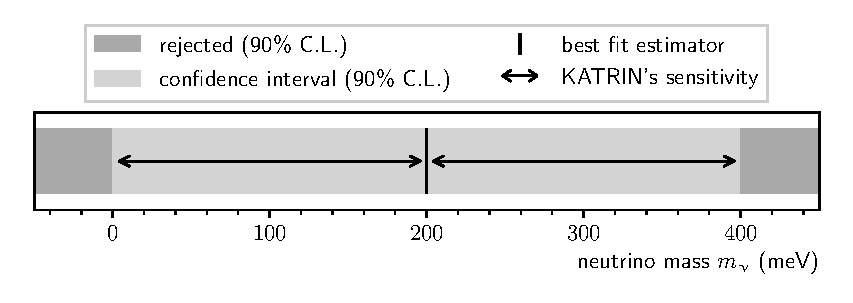
\includegraphics[width=\textwidth]{\currentFigureFolder/sensitivityIllustration.pdf}
	\xcaption{Illustration of KATRIN's sensitivity to the neutrino mass}{Illustration of KATRIN's sensitivity to the neutrino mass.}{The graph illustrates KATRIN's sensitivity of~\SI{200}{meV}~\cite{Angrik:2005ep} as per equation~\eqref{eq:statMethodsSensitivity}. It shows a hypothetical measurements of to the neutrino mass with a symmetric confidence interval \mbox{(\SI{90}{\percent} C.L.)} centrally located around the best fit estimator. If such a classical confidence interval is constructed, KATRIN can reject the null hypothesis of a vanishing neutrino mass at \mbox{\SI{90}{\percent} C.L.} if it estimates a neutrino mass of at least~\SI{200}{meV}.}
	\label{fig:statMethodsSensitivity}
\end{figure}

KATRIN's sensitivity can be understood as half the width of a symmetric and central confidence interval (\SI{90}{\percent} C.L.) for the neutrino mass obtained from a KATRIN neutrino mass measurement. As such it can be constructed from a 1-$\sigma$ uncertainty $\totUncert$ on the squared neutrino mass~\cite{Angrik:2005ep}
\begin{equation}
\label{eq:statMethodsSensitivity}
S_{\nuMass}(\SI{90}{\percent}) = \sqrt{1.645\cdot\totUncert}
\comma
\end{equation}
where the factor 1.645 translates the $\SI{68.3}{\percent}$ interval into a $\SI{90}{\percent}$ interval.

In other words, KATRIN's sensitivity to the neutrino mass can be understood as the minimal neutrino mass that has to be inferred from a KATRIN neutrino mass measurement to exclude the null hypothesis of a vanishing neutrino mass~\cite{Kleesiek2014} when constructing a symmetric and central confidence interval (\SI{90}{\percent} C.L.). Figure~\ref{fig:statMethodsSensitivity} illustrates this statement.

For a more comprehensive picture, where not only a symmetric and central confidence interval is considered, but also the unified approach according to Feldmann and Cousins as well as Bayesian statistics, the reader is referred to~\cite{Kleesiek2019}.

\subsection{Sensitivity from Simulated Ensembles}
\label{sec:statMethodsSensitivtyFromEnsemble}
In the KATRIN Design Report the sensitivity to the neutrino mass was evaluated using ensemble tests. An ensemble of many KATRIN measurements was simulated (see section~\ref{sec:intSpecModelNuMassMeasurement} on how such a simulation can be conducted) with a true neutrino mass of \SI{0}{eV}. From each simulated measurement the squared neutrino mass was inferred in a standard KATRIN four-parameter fit (see section~\ref{sec:statMethodsStandardFit}). Probability was interpreted as the frequency of an outcome of such a fit. The central 1-$\sigma$ interval of the obtained ensemble of squared neutrino masses was taken as the statistical uncertainty on the squared neutrino mass~\cite{Angrik:2005ep}
\begin{equation}
	\statUncertTDR = \SI{0.018}{eV^2}
\end{equation}
A systematic uncertainty was estimated to be approximately \SI{0.01}{eV}. Due to the early stage of the experiment the systematic uncertainty was conservatively enlarged to a systematic budget at approximately the same scale as the statistical uncertainty~\cite{Angrik:2005ep}
\begin{equation}
	\sysUncertTDR = \SI{0.017}{eV^2}
\end{equation}
Adding the statistic and systematic uncertainty quadratically and applying the definition~\eqref{eq:statMethodsSensitivity} yields KATRIN's design sensitivity~\cite{Angrik:2005ep}
\begin{equation}
	\label{eq:statMethodsSensitivityDesignReport}
	S_{\nuMass}^{\mathrm{TDR}}(\SI{90}{\percent}) = 
	\sqrt{1.645\cdot
		\sqrt{
		\statUncertTDR^2+\sysUncertTDR^2
	}}
	\approx \SI{200}{meV}
	\fullstop
\end{equation}
The corresponding investigations were redone in the scope of several works. Table~\ref{tab:statMethodsSensitivityFromEnsembleTests} lists selected results.
\begin{table}[tb]
	\centering
	\xcaption{KATRIN's sensitivity to the neutrino mass from ensemble tests}{KATRIN's sensitivity to the neutrino mass from ensemble tests.}{The table lists KATRIN's sensitivity~$S_{\nuMass}(\SI{90}{\percent})$ as defined by equation~\eqref{eq:statMethodsSensitivity}. Several works reevaluated the statistical uncertainty according to experimental and theoretical progress. For each reevaluation a systematic uncertainty of $\sysUncert = \SI{0.017}{eV^2}$ was assumed. A value derived from an ensemble test is a random variable. Corresponding uncertainty intervals are reprinted where originally stated.}
	\begin{tabular}{lrlr}
		\toprule
		\makecell[t]{$\statUncert$ (\SI{}{eV^2})} & 
		\makecell[t]{$S_{\nuMass}(\SI{90}{\percent})$ (\SI{}{meV})} & 
		\makecell[t]{comment} &
		\makecell[t]{reference}
		\\
		\hline
		0.018 & 200 & design value & \cite{Angrik:2005ep} \\
		$0.0165\pm0.0001$ & 198 & updated $\upbeta$-spectrum calculation & \cite{Hoetzel2012} \\
		$0.0162\pm0.0001$ & 197 & further updated $\upbeta$-spectrum calculation & \cite{Kleesiek2014} \\
		0.01490 & 193 & optimized \gls{mtd} & \cite{Kleesiek2014} \\
		\bottomrule
	\end{tabular}
	\label{tab:statMethodsSensitivityFromEnsembleTests}
\end{table}
\subsection{Sensitivity from  the Profile-Likelihood Method}
\label{sec:statMethodsSensitivtyFromProileLikelihood}
In the scope of this thesis, the sensitivity on the neutrino mass as obtained by the profile-likelihood method is of importance. (See chapter~\ref{sec:katrinEloss} for a description and application of the profile-likelihood method.) In this regard, previous results from~\cite{Kleesiek2014} based on the profile-likelihood method are shortly reviewed here. Two uncertainties were obtained for two different~\gls{mtd}s in a KATRIN standard 4-parameter fit (see section~\ref{sec:statMethodsStandardFit}). The first \gls{mtd} had been specially optimized with regard to KATRIN's sensitivity and the resulting statistical uncertainty is $\statUncert=\SI{0.01494}{eV^2}$. For the second result the nominal \gls{mtd} from the KATRIN Design Report was used as introduced in section~\ref{sec:intSpecModelMTD}. The corresponding profile likelihood was plotted and $\statUncert$ can be extracted to be between \SIrange[range-phrase=--]{0.0155}{0.0165}{eV^2}. Both results are in agreement on the $10^{-3}$ level with the results from ensemble tests (see~\cite{Kleesiek2014} in table~\ref{tab:statMethodsSensitivityFromEnsembleTests}). This is an indicator for the general validity of the profile-likelihood method in the context of a KATRIN measurement. A more detailed discussion on the matter is given in chapter~\ref{sec:katrinEloss}.